%%%%%%%%%%%%%%%%%%%%%%%%%%%%%
% Standard header for working papers
%
% WPHeader.tex
%
%%%%%%%%%%%%%%%%%%%%%%%%%%%%%

\documentclass[11pt]{article}

%%%%%%%%%%%%%%%%%%%%
%% Include general header where common packages are defined
%%%%%%%%%%%%%%%%%%%%

% general packages without options
\usepackage{amsmath,amssymb,bbm}




%%%%%%%%%%%%%%%%%%%%
%% Idem general commands
%%%%%%%%%%%%%%%%%%%%
%% Commands

\newcommand{\noun}[1]{\textsc{#1}}


%% Math

% Operators
\DeclareMathOperator{\Cov}{Cov}
\DeclareMathOperator{\Var}{Var}
\DeclareMathOperator{\E}{\mathbb{E}}
\DeclareMathOperator{\Proba}{\mathbb{P}}

\newcommand{\Covb}[2]{\ensuremath{\Cov\!\left[#1,#2\right]}}
\newcommand{\Eb}[1]{\ensuremath{\E\!\left[#1\right]}}
\newcommand{\Pb}[1]{\ensuremath{\Proba\!\left[#1\right]}}
\newcommand{\Varb}[1]{\ensuremath{\Var\!\left[#1\right]}}

% norm
\newcommand{\norm}[1]{\| #1 \|}


% amsthm environments
\newtheorem{definition}{Definition}



%% graphics

% renew graphics command for relative path providment only ?
%\renewcommand{\includegraphics[]{}}








% geometry
\usepackage[margin=2cm]{geometry}

% layout : use fancyhdr package
\usepackage{fancyhdr}
\pagestyle{fancy}

\makeatletter

\renewcommand{\headrulewidth}{0.4pt}
\renewcommand{\footrulewidth}{0.4pt}
%\fancyhead[RO,RE]{\textit{Working Paper}}
\fancyhead[RO,RE]{\textit{ECTQG 2015}}
%\fancyhead[LO,LE]{G{\'e}ographie-Cit{\'e}s/LVMT}
\fancyhead[LO,LE]{An Algorithmic Systematic Review}
\fancyfoot[RO,RE] {\thepage}
\fancyfoot[LO,LE] {\noun{J. Raimbault}}
\fancyfoot[CO,CE] {}

\makeatother


%%%%%%%%%%%%%%%%%%%%%
%% Begin doc
%%%%%%%%%%%%%%%%%%%%%

\begin{document}







\title{Génération de Données Synthétiques Corrélées\\\medskip
\textit{Actes des Journées de Rochebrune 2016}
}
\author{\noun{Juste Raimbault}$^{1,2}$\\
$^{1}$ UMR CNRS 8504 Géographie-cités\\
$^{2}$ UMR-T IFSTTAR 9403 LVMT
}
\date{date}


\maketitle

\justify


\begin{abstract}
\end{abstract}



%%%%%%%%%%%%%%%%%%%%%%
\section{Introduction}
%%%%%%%%%%%%%%%%%%%%%%

L'utilisation de données synthétiques, au sens de populations statistiques d'individus générées aléatoirement sous la contrainte de reproduire certaines caractéristiques du système étudié, est une pratique méthodologique largement répandue dans de nombreuses disciplines, et particulièrement pour des problématiques liées aux systèmes complexes, telles que par exemple l'évaluation thérapeutique~\cite{abadie2010synthetic}, l'étude des systèmes territoriaux~\cite{moeckel2003creating,pritchard2009advances}, l'apprentissage statistique~\cite{bolon2013review} ou la bio-informatique~\cite{van2006syntren}. Il peut s'agir d'une désagrégation par création d'une population au niveau microscopique présentant des caractéristiques macroscopiques données, ou bien de la création de nouvelles populations au même niveau d'agrégation qu'un échantillon donné avec un critère de ressemblance aux données réelles. Le niveau de ce critère peut % find minimal common characteristics ?
% TODO generalization of data proximity

Les intérêts de ces méthodes sont directement liés 



Si le premier ordre est bien maitrisé, il n'a à notre connaissance pas été proposé de méthode systématique permettant un contrôle au second ordre,% rq correlated choices in DC model ?
c'est à dire où la structure de correlation estimée sur les données générées est maitrisée. Nous proposons une telle méthode ainsi que son application à deux exemples de systèmes complexes dans des domaines relativement éloignés.

La suite de l'article est organisée de la façon suivante : 


%%%%%%%%%%%%%%%%%%%%%%
\section{Formalisation de la méthode}
%%%%%%%%%%%%%%%%%%%%%%

L'ensemble des méthodologies mentionnées en introduction sont trop variées pour être résumées par un même formalisme. Nous proposons ici une formulation générique ne dépendant pas du domaine d'application, ciblée sur le contrôle de la structure de correlation des données synthétiques.

Soit un processus stochastique multidimensionnel $\vec{X}_I$ (l'ensemble d'indexation pouvant être par exemple le temps dans le cas de séries temporelles, l'espace, ou l'indexation). On se propose, à partir d'un jeu de réalisations $\mathbf{X}=(X_{i,j})$, de générer une population statistique $\mathbf{\tilde{X}}=\tilde{X}_{i,j}$ telle que
\begin{itemize}
\item d'une part un certain critère de proximité aux données est vérifié, i.e. étant donné une précision $\varepsilon$ et un indicateur $f$, $\norm{f(\mathbf{X})-f(\mathbf{\tilde{X}})} < \varepsilon$
\item d'autre part le niveau de correlation est controlé, i.e. étant donné une matrice fixant une structure de covariance $R$, $\Varb{(\tilde{X}_i)} = R$, où la matrice de variance/covariance est estimée sur la population synthétique.
\end{itemize}


%%%%%%%%%%%%%%%%%%%%%%
\section{Applications}
%%%%%%%%%%%%%%%%%%%%%%



%%%%%%%%%%%%%%%%%%%%%%
\subsection{Application : séries temporelles financières}


%%%%%%%%%%%%%%%%%%%%%%
\subsubsection{Contexte}

Un premier domaine d'application proposé pour notre méthode est celui des séries temporelles financières, signaux typiques de systèmes complexes hétérogènes et multiscalaires~\cite{mantegna2000introduction} et pour lesquels les corrélations ont fait l'objet d'abondants travaux. Ainsi, l'application de la théorie des matrices aléatoires peut permettre de débruiter, ou du moins d'estimer la part de signal noyée dans le bruit, une matrice de correlations pour un grand nombre d'actifs échantillonnés à faible fréquence (retours journaliers par exemple)~\cite{2009arXiv0910.1205B}. De même, l'analyse de réseaux complexes construits à partir des corrélations, selon des méthodes type arbre couvrant minimal~\cite{2001PhyA..299...16B} ou des extensions raffinées pour cette application précise~\cite{tumminello2005tool}, ont permis d'obtenir des résultats prometteurs, tels la reconstruction de la structure économique des secteurs d'activités. A haute fréquence, l'estimation précise de paramètres d'interdépendance dans le cadre d'hypothèses fixées sur la dynamique, fait l'objet d'importants travaux théoriques dans un but de raffinement théorique des estimateurs~\cite{barndorff2011multivariate}. Les résultats théoriques doivent alors être testés sur des jeux de données synthétiques, qui permettent de contrôler un certain nombre de paramètres et de s'assurer qu'un effet prédit par la théorie est bien observable \emph{toutes choses égales par ailleurs}. Par exemple, \cite{potiron2015estimation} dérive une correction du biais de l'estimateur de \emph{Hayashi-Yoshida} qui est un estimateur de la covariance de deux browniens corrélés à haute fréquence dans le cas de temps d'observation asynchrones, par démonstration d'un théorème de la limite centrale pour un modèle généralisé endogénéisant les temps d'observations. La confirmation empirique de l'amélioration de l'estimateur est alors obtenue sur un jeu de données synthétiques à un niveau de corrélation fixé.


%%%%%%%%%%%%%%%%%%%%%%
\subsubsection{Formalisation}

\paragraph{Cadre}

Considérons un réseau d'actifs $(X_i(t))_{1\leq i \leq N}$ échantillonnés à haute fréquence (typiquement 1s). On se place dans un cadre multi-scalaire (utilisé par exemple dans les approches par ondelettes~\cite{ramsey2002wavelets} ou analyses multifractales du signal~\cite{bouchaud2000apparent}) pour interpréter les signaux observés comme la superposition de composantes à des multiples échelles temporelles : $X_i=\sum_{\omega}{X_i^{\omega}}$. Prédire l'évolution d'une composante à une échelle donnée est alors un problème caractéristique de l'étude des systèmes complexes, pour lequel l'enjeu est l'identification de régularités et leur distinction des composantes considérées comme stochastiques en comparaison. Dans un souci de simplicité, on représente un tel processus par un modèle de prédiction de tendance à une échelle temporelle $\omega_1$ donnée, formellement un estimateur $M_{\omega_1} : (X_i(t'))_{t'<t} \mapsto \hat{X_i}(t)$ dont l'objectif est la minimisation de l'erreur sur la tendance réelle $\norm{X_i^{\omega}}$. Dans le cas d'estimateurs auto-regressifs multivariés, la performance dépendra entre autre des correlations respectives entre actifs et il est alors intéressant d'utiliser la méthode pour évaluer celle-ci en fonction de niveaux de correlation à plusieurs échelles. On assume une dynamique de Black-Scholes~\cite{jarrow1999honor} pour les actifs, i.e. $dX = \sigma\cdot dW$ avec $W$ processus de Wiener, ce qui permettra d'obtenir facilement des niveaux de correlation voulus.

\paragraph{Génération des données}

Il est alors aisé de générer $\tilde{X}_i$ tel que $\Varb{\tilde{X}_i^{\omega_0}}=\Sigma R$ ($\Sigma$ variance estimée et $R$ matrice de corrélation fixée), par la simulation de processus de Wiener au niveau de corrélation fixé et tel que $X_i^{\omega < \omega_0} = \tilde{X}_i^{\omega < \omega_0}$ (critère de proximité au données : les composantes à plus basse fréquence sont identiques). En effet, si $dW_1 \indep dW_1^{\indep}$, alors $W_2 = \rho_{12}W_1 + \sqrt{1-\frac{\sigma_1^2}{\sigma_2^2}\cdot\rho_{12}^2}W_1^{\indep}$ est tel que $\rho(dW_1,dW_2)=\rho_{12}$. Les signaux suivants sont construits de la même manière par orthonormalisation de Gram. On isole alors la composante de la première fréquence $\omega_1 < \omega_0$ par filtrage, et on reconstruit les signaux synthétiques par $\tilde{X}_i = [\sum_{\omega<\omega_1}X_i^{\omega}]+\tilde{X}_i^{\omega_0}$.
% TODO pb signal reconstruction, clarify formalisation.


\subsubsection{Implémentation et Résultats}

\paragraph{Méthodologie}

La méthode est testée sur un exemple de deux actifs du marché des devises (EUR/USD et EUR/GBP), sur une période de 6 mois de juin 2015 à novembre 2015. Le nettoyage des données\footnote{obtenues depuis \texttt{http://www.histdata.com/}, sans licence spécifiée, les données nettoyées et filtrées à $\omega_m$ uniquement sont mises en accessibilité pour respect du copyright.}, originellement échantillonnées à l'ordre de la seconde, consiste dans un premier temps à la détermination du support temporel commun maximal (les séquences manquantes étant alors ignorées, par translation verticale des séries, i.e. $S(t):=S(t)\cdot \frac{S(t_{n})}{S(t_{n-1})}$ lorsque $t_{n-1},t_n$ sont les extrémités du ``trou'' et $S(t)$ la valeur de l'actif, ce qui revient à garder la contrainte d'avoir des retours à pas de temps similaires entre actifs). On étudie alors les \emph{log-prix} et \emph{log-retours}, définis par $X(t):=\log{\frac{S(t)}{S_0}}$ et $\Delta X (t) = X(t) - X(t-1)$. Les données brutes sont filtrées à une fréquence $\omega_m = 10\textrm{min}$ (qui sera la fréquence maximale d'étude) pour un souci de performance computationnelle. On fixe $\omega_0=12\textrm{h}$ et on se propose de construire des données synthétiques aux fréquences $\omega_1 = 30\textrm{min},1\textrm{h},2\textrm{h}$. Il est crucial de noter l'interférence entre les fréquences $\omega_0$ et $\omega_1$ dans le signal construit : la correlation effectivement estimée est
\[
\rho_{e} = \rho \left[ \Delta \tilde{X}_1 , \Delta \tilde{X}_2 \right] = \rho \left[ X_1^{\omega_0} + \sum_{\omega_0 < \omega < \omega_1} \tilde{X}_1^{\omega} ,  X_2^{\omega_0} + \sum_{\omega_0 < \omega < \omega_1} \tilde{X}_2^{\omega}\right]
\]
ce qui conduit à dériver dans la limite raisonnable $\sigma_1 \gg \sigma_0$ (fréquence fondamentale suffisamment basse), lorsque $\Covb{\tilde{X}_i^{\omega}}{X_j^{\omega_0}}=0$ pour tous $i,j,\omega > \omega_0$, en notant $\rho_0 = \rho \left[X_1^{\omega_0} , X_2^{\omega_0} \right]$, $\rho = \rho \left[ \sum_{\omega_0 < \omega < \omega_1} \tilde{X}_1^{\omega} , \sum_{\omega_0 < \omega < \omega_1} \tilde{X}_2^{\omega} \right]$, et $\varepsilon_i = \frac{\sigma (X_i^{\omega_0})}{\sigma \left( \sum_{\omega_0 < \omega < \omega_1} \tilde{X}_i^{\omega}\right)}$, la correction sur la correlation effective due aux interférences : le correlation effective est alors au premier ordre :

\begin{equation}
\label{eq:}
\rho_e = \varepsilon_1 \varepsilon_2 \rho_0 + \rho 
\end{equation}

 la correction sur la correlation

% TODO : explain which estimator

% TODO : formalize arma model.


\paragraph{Implémentation}

L'implémentation est faite en language R, utilisant en particulier la bibliothèque \texttt{MTS}~\cite{Tsay:2015xy} pour les modèles de séries temporelles. Les données nettoyées et le code source sont disponibles de manière ouverte sur le dépôt \texttt{git} du projet\footnote{at \texttt{https://github.com/JusteRaimbault/SynthAsset}}.

\paragraph{Résultats}

La figure~\ref{fig:effective_corrs} donne les correlations effectives calculées sur les données synthétiques.
% comment

% fig:model_perf : application à la perf de l'arma.

% implication thématiques et développements possibles


%%%%%%%%%%%%%%%%%%%
\begin{figure}
\centering
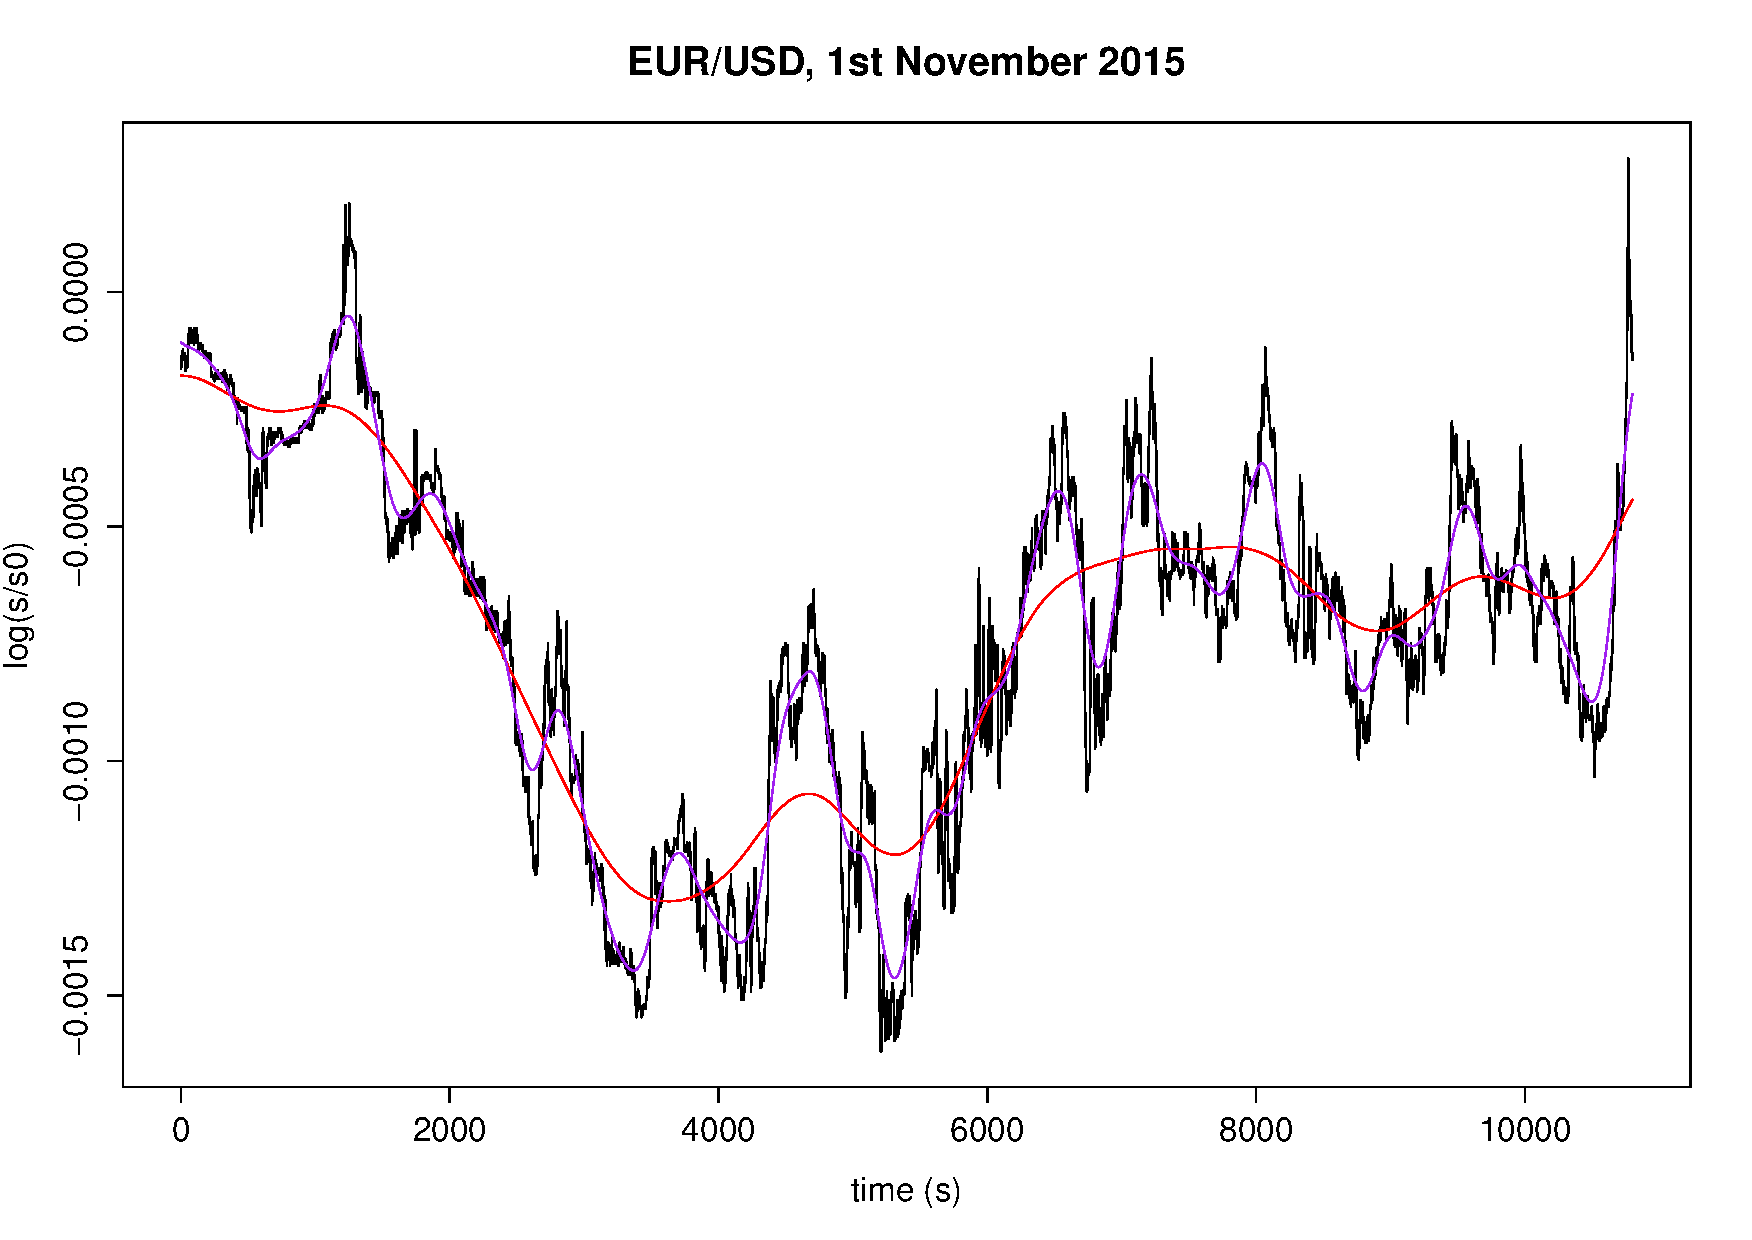
\includegraphics[width=0.7\textwidth]{figures/asset/ex_filtering}
\caption{\textbf{Exemple de la structure multi-scalaire du signal qui sert de base à la construction des signaux synthétiques | } Les \emph{log-prix} sont représentés sur environ 3h pour la journée du 1er novembre 2015 pour l'actif EUR/USD, ainsi que les tendances à 10min (violet) et à 30min.}
\label{fig:example_signal}
\end{figure}
%%%%%%%%%%%%%%%%%%%




%%%%%%%%%%%%%%%%%%%
\begin{figure}
\centering
% figure : effective correlations, with confidence intervals (bootstrap), for the 3 filtering scales. ; AND expected corrected corrs from derivation above.
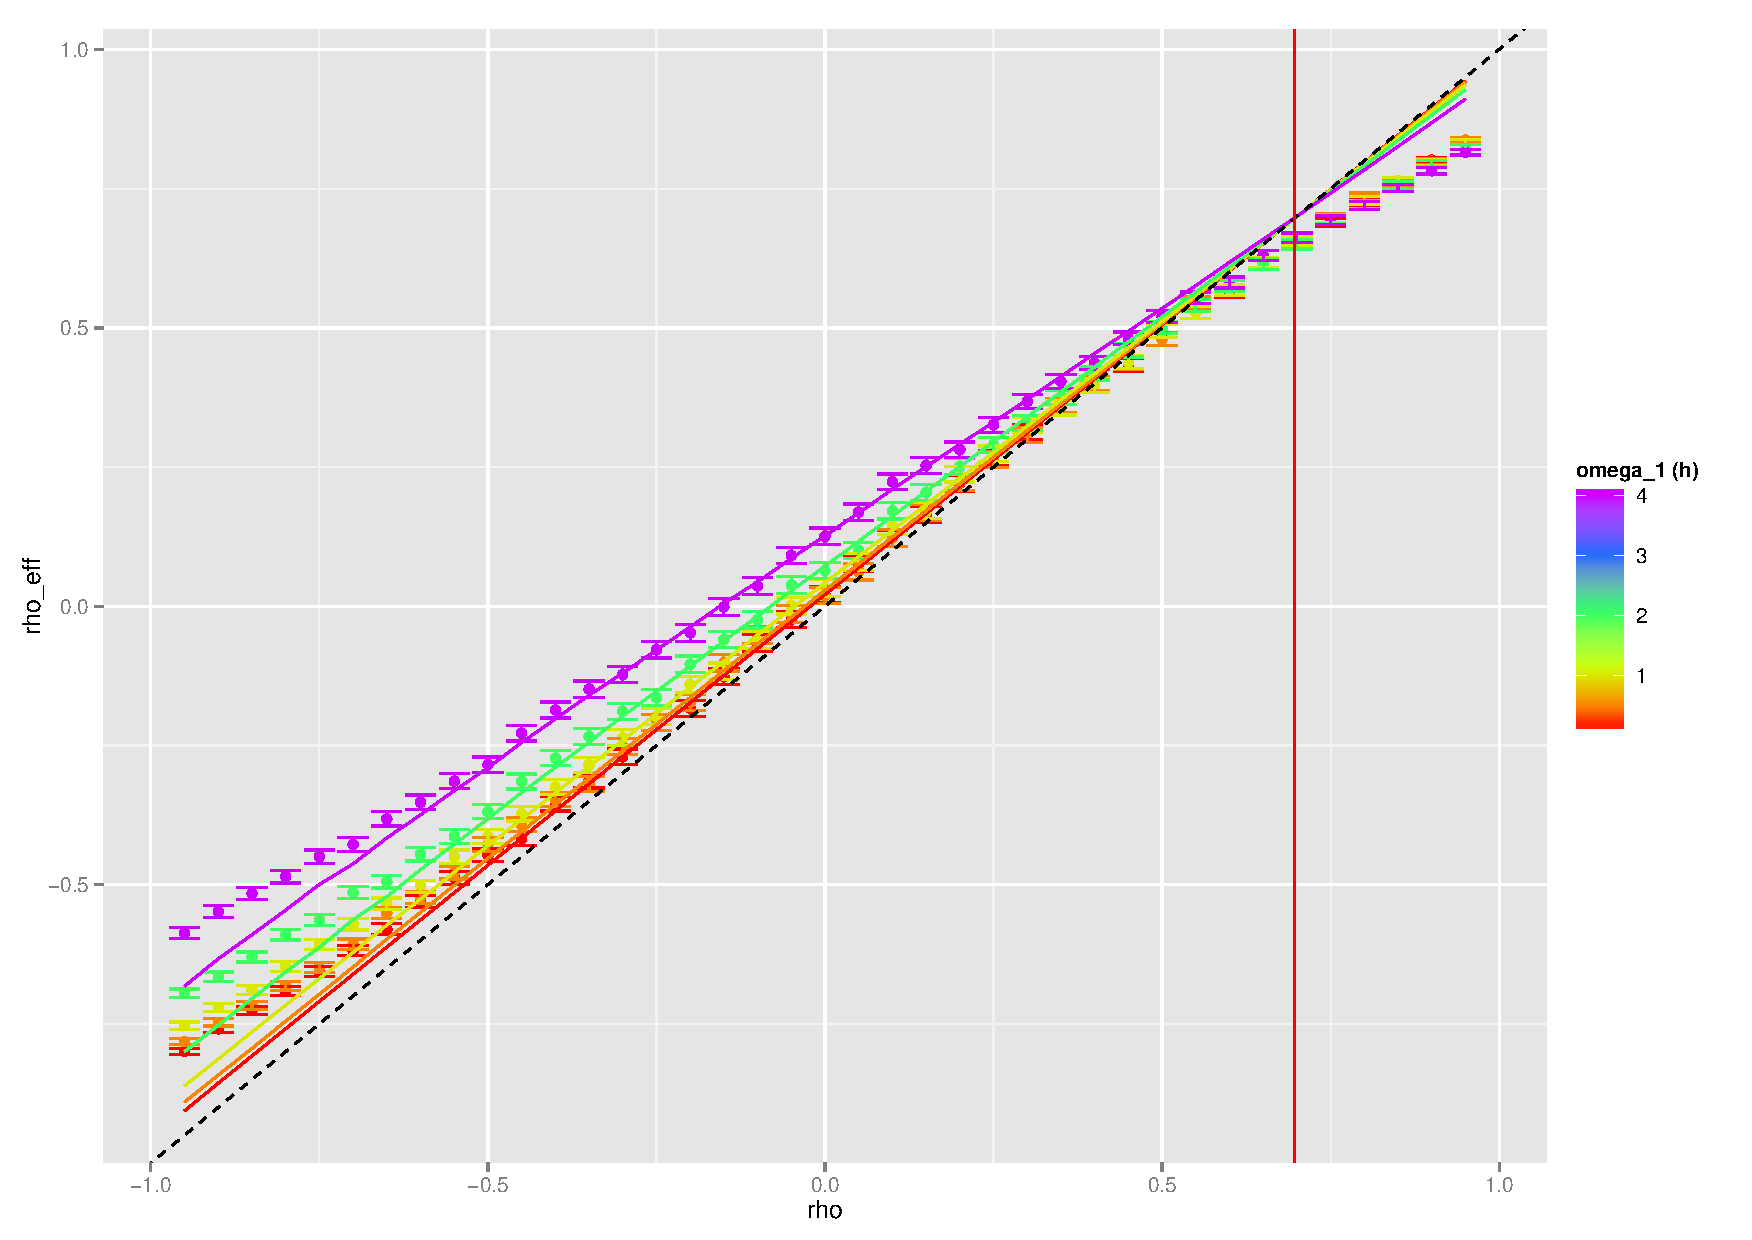
\includegraphics[width=0.7\textwidth]{figures/effectiveCorrs_withGoodTh_A4}
\caption{\textbf{Correlations effectives obtenues sur les données synthétiques | } Les points représentent les correlations estimées sur une génération d'un jeu de données synthétiques correspondant aux 6 mois de juin à novembre 2015 (barres d'erreurs obtenue par méthode de Fisher standard) ; l'échelle de couleur donne la fréquence de filtrage $\omega_1=10\textrm{min},30\textrm{min},1\textrm{h},2\textrm{h},4\textrm{h}$ ; les courbes sont les valeurs théoriques de $\rho_e$}
\label{fig:effective_corrs}
\end{figure}
%%%%%%%%%%%%%%%%%%%


%%%%%%%%%%%%%%%%%%%
\begin{figure}
% figure : performance of arma2 as a function of expected correlation.

\caption{}
\label{fig:model_perf}
\end{figure}
%%%%%%%%%%%%%%%%%%%





%%%%%%%%%%%%%%%%%%%%%%
\subsection{Application : données géographiques de densité et de réseaux}


%%%%%%%%%%%%%%%%%%%%%%
\subsubsection{Contexte}


En géographie, l'utilisation de données synthétiques est plus généralement axée vers l'utilisation de population synthétiques au sein de modèles basés agents (mobilité, modèles \emph{LUTI})~\cite{pritchard2009advances}. Il a récemment été proposé de contrôler systématiquement les effets de la configuration spatiale sur le comportement de modèles de simulation spatialisés~\cite{cottineau2015revisiting}, méthodologie pouvant être interprétée comme un contrôle par données statistiques spatiales. L'enjeu est de pouvoir alors distinguer effets propres dus à la dynamique intrinsèque du modèle, d'effet particuliers dus à la structure géographique du cas d'application. Celui-ci est crucial pour la validation des conclusions issues des pratiques de modélisation et simulation en géographie quantitative.


%%%%%%%%%%%%%%%%%%%%%%
\subsubsection{Formalisation}

Dans notre cas, nous proposons de générer des systèmes de villes représentés par une densité spatiale de population $d(\vec{x})$ et la donnée d'un réseau de transport $n(\vec{x})$, représenté de façon simplifiée, pour lesquels on serait capable de contrôler les correlations entre mesures morphologiques de la densité urbaine et caractéristiques du réseau. Nous proposons un couplage \emph{simple}


\paragraph{Modèle de densité}

L'utilisation d'un modèle $D$ type aggrégation-diffusion~\cite{batty2006hierarchy} permet de générer une distribution discrete de densité. Dans \cite{}, %cit Working Paper ?
une généralisation de ce modèle est calibré pour des objectifs morphologiques $M$ (entropie, hiérarchie, auto-corrélation spatiale, distance moyenne) contre les valeurs réelles calculées sur l'ensemble des grilles de taille 50km extraites de la grille européenne de densité~\cite{eurostat}. Plus précisément, le modèle fonctionne de manière itérative de la façon suivante. Une grille initialement vide de côté $N$, est représentée par la données des populations $(P_i(t))_{1\leq i\leq N^2}$. A chaque pas de temps, jusqu'à ce que la population atteigne une valeur fixée $P_m$,
\begin{itemize}
\item la population totale $P(t)$ est augmentée d'un nombre fixé $N_G$ (taux de croissance), suivant un attachement préférentiel tel que $\Pb{P_i(t+1)=P_i(t)+1|P(t+1)=P(t)+1}=\frac{(P_i(t)/P(t))^{\alpha}}{\sum(P_i(t)/P(t))^{\alpha}}$
\item une diffusion d'une fraction $\beta$ de la population aux 4 plus proches voisins est effectuée $n_d$ fois
\end{itemize}

Les deux processus antagonistes de concentration et d'étalement urbain sont capturés par le modèle, ce qui permet de reproduire assez fidèlement un grand nombre de morphologies existantes.


\paragraph{Modèle de réseau}

D'autre part, on est capable de générer par un modèle $N$ un réseau de transport planaire à une échelle équivalente, étant donné une distribution de densité. La génération du réseau étant conditionnée à la donnée de la densité, les estimateurs des indicateurs de réseau seront nécessairement conditionnels d'une part, et d'autre part les formes urbaines et du réseau devraient nécessairement être correlées, les processus n'étant pas indépendants. La nature et la modularité de ces correlations selon la variation des paramètres des modèles restent à déterminer par l'exploration du modèle couplé.

La procédure de génération heuristique de réseau est la suivante :
\begin{itemize}
\item Une nombre fixé $N_c$

\end{itemize}

On distribue un nombre fixé de noeuds de manière aléatoire en suivant la loi de probabilité spatiale donnée par les valeurs de densité, puis un algorithme déterministe de connexification permet d'obtenir un réseau arborescent. Le réseau est ensuite étendu par la création de boucles locales dans un rayon de voisinage $r_l$ ainsi que de raccourcis à une plus grande échelle $r_g$, aléatoirement selon un processus de rupture des potentiels gravitaires\footnote{Notons que ce choix est heuristique, et que d'autres types de modèles type réseau biologique auto-généré~\cite{tero2006physarum} par exemple pourraient également être envisagés, dans l'idée d'une architecture modulaire où le choix entre différentes implémentations d'une brique fonctionnelle peut être vue comme méta-paramètre~\cite{cottineau2015incremental}.}.


% detail network generation process

% idea -> generate continuous center distribution given density as proba distribution ; tree-connexify network deterministically ; apply local loops and gravity-based adjustements. (check params to have enough degrees of freedom for a custom of global network measures. diameter or euclidian perf ?




\paragraph{Espace des paramètres}






%%%%%%%%%%%%%%%%%%%%%%
\subsubsection{Implémentation}

Le couplage des modèles génératifs est effectué à la fois au niveau formel et au niveau opérationnel 



%%%%%%%%%%%%%%%%%%%%%%
\subsubsection{Résultats}

L'étude du modèle de densité est développée dans~\cite{}.% TODO



%%%%%%%%%%%%%%%%
\begin{figure}
% figure : density example, exploration and calibration ?


\end{figure}
%%%%%%%%%%%%%%%%


A densité fixée, les premières explorations de l'espace des paramètres du modèle de réseau synthétique suggèrent une assez bonne flexibilité sur des indicateurs globaux $G$ (diamètre, longueur cumulée, centralité moyenne, degré moyen). L'exploration systématique via le logiciel OpenMole~\cite{reuillon2013openmole} par calcul intensif est un travail en cours, ainsi que la calibration contre les mesures réelles calculées sur l'ensemble de l'Europe sur des zones identiques au modèle de densité, via les données de réseau routier d'OpenStreetMap. La connaissance très fine ainsi obtenue du comportement de $N$ (distribution statistiques sur une grille fine de l'espace des paramètres à trois dimensions), devrait permettre, étant donné une population de configuration de densités $\tilde{D}$, de déterminer via $N^{<-1>}$ une population de réseau $\tilde{N}$ telle que $\Covb{M}{G}$ a une structure fixée (via la détermination de la valeur des paramètres à utiliser pour chaque individu de $\tilde{D}$). On pourra éventuellement appliquer des algorithmes plus fins d'exploration pour atteindre des configurations exceptionelles réalisant un niveau de corrélation voulu~\cite{10.1371/journal.pone.0138212}. Les indicateurs globaux devraient ainsi être corrélés à un niveau contrôlé, tandis que les densités et réseaux restent cohérents dans l'espace de par la forme du réseau, conditionnelle à la distribution de densité. Les applications géographiques potentielles de cette implémentation de la méthode incluent le contrôle statistique de l'effet des corrélations entre ville et réseaux sur des modèles de simulation spatiaux par exemple.



%%%%%%%%%%%%%%
\begin{figure}

\begin{subfigure}[t]{0.35\linewidth}
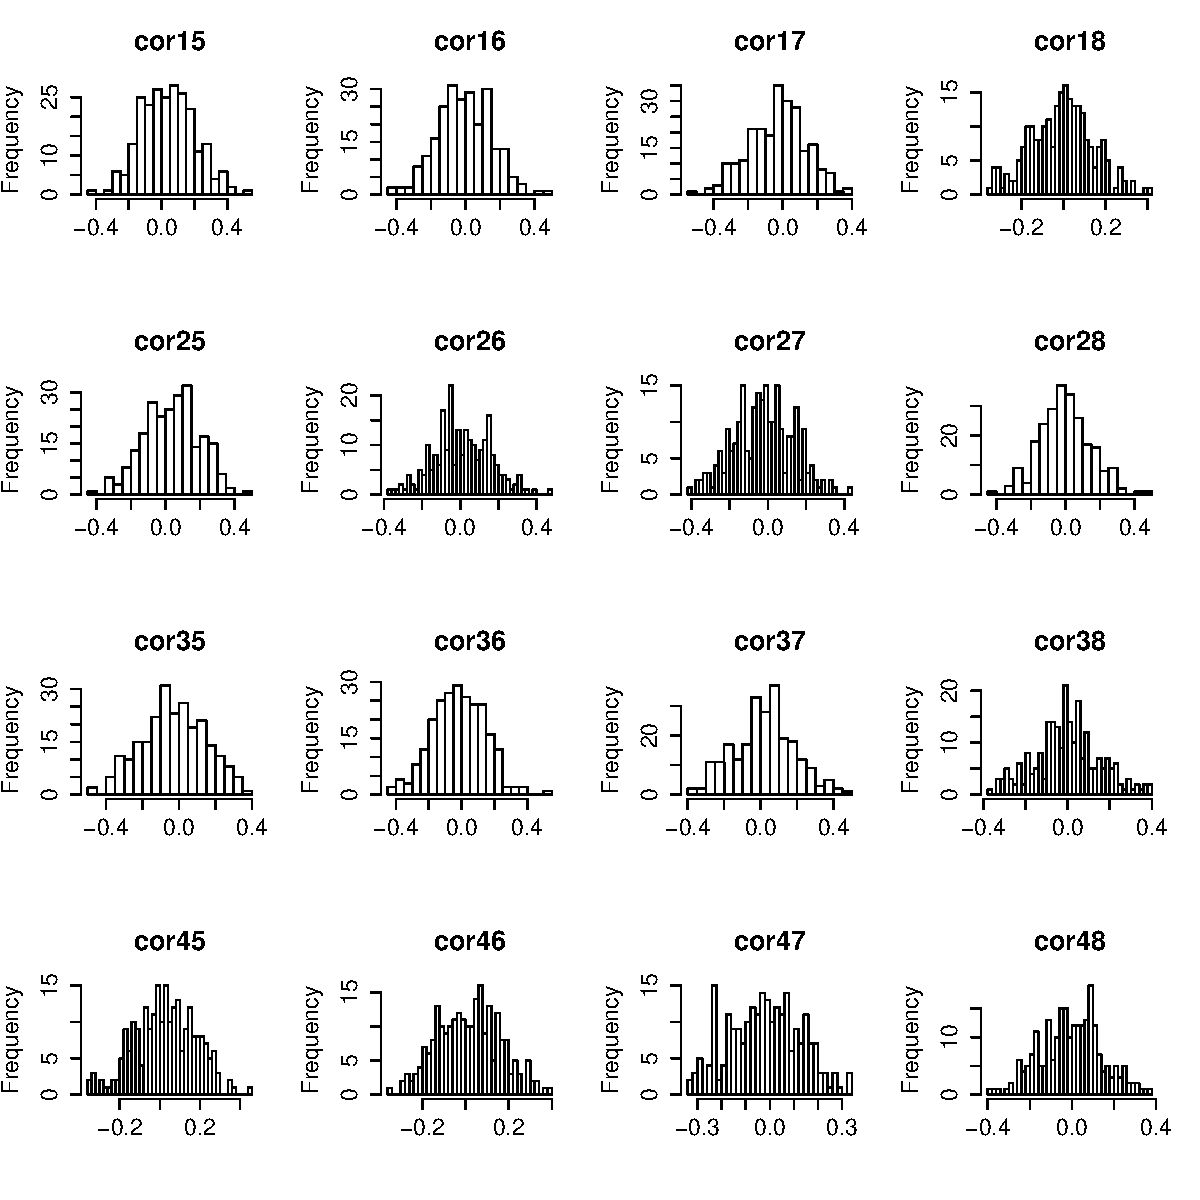
\includegraphics[width=\textwidth]{figures/hist_crossCorMat}
\caption{}
\end{subfigure}
\begin{subfigure}[t]{0.23\linewidth}
\vspace{-6.5cm}
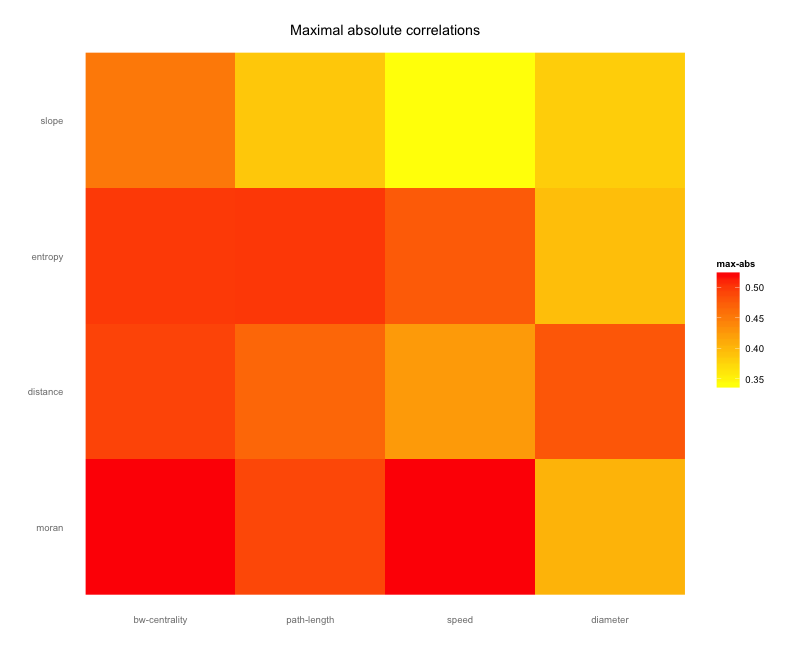
\includegraphics[width=\textwidth]{figures/heatmap_maxAbsCor}\\
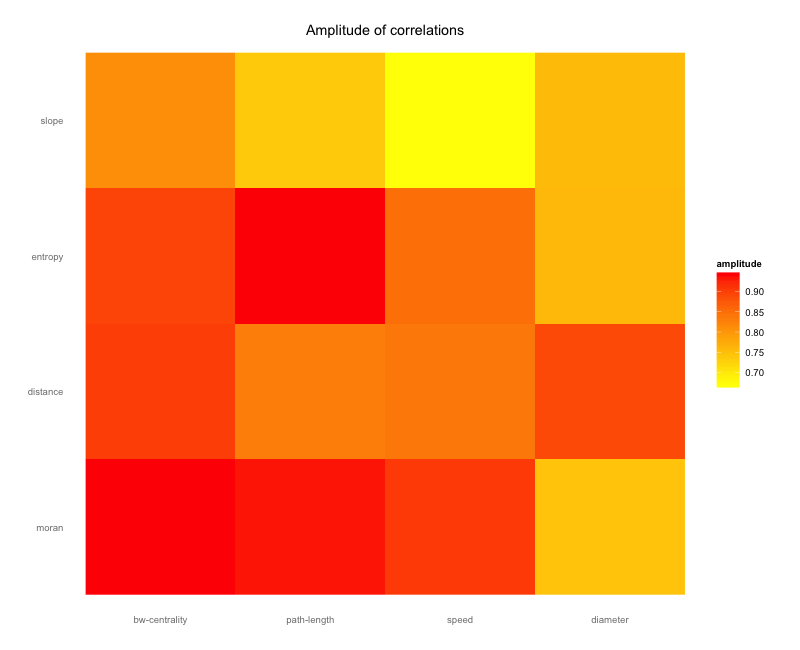
\includegraphics[width=\textwidth]{figures/heatmap_amplCor}
\caption{}
\end{subfigure}
\begin{subfigure}[t]{0.4\linewidth}
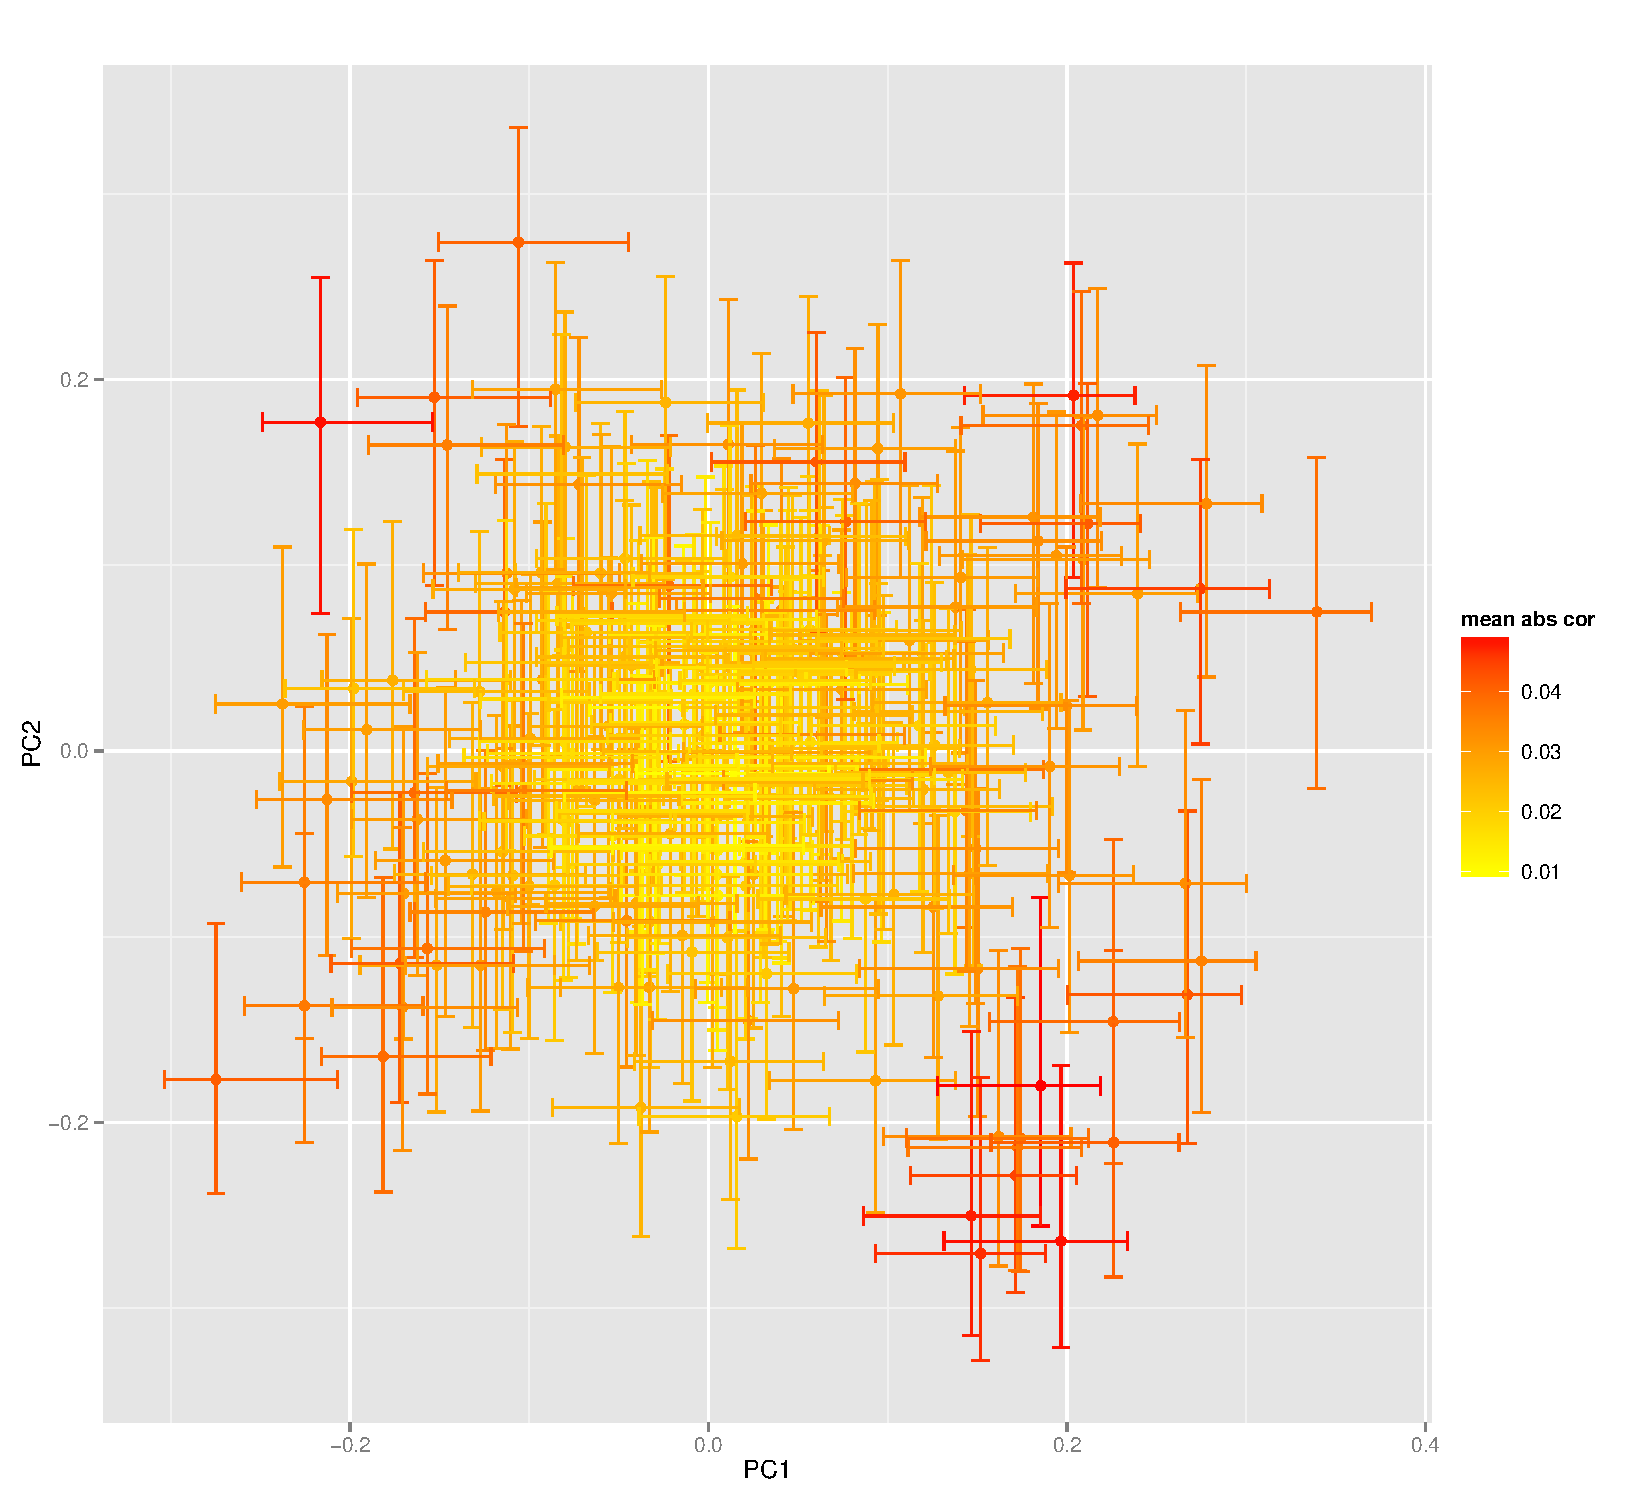
\includegraphics[width=\textwidth]{figures/pca_meanAbsCor_errorBars}
\caption{}
\end{subfigure}\\
\begin{subfigure}[t]{0.54\linewidth}
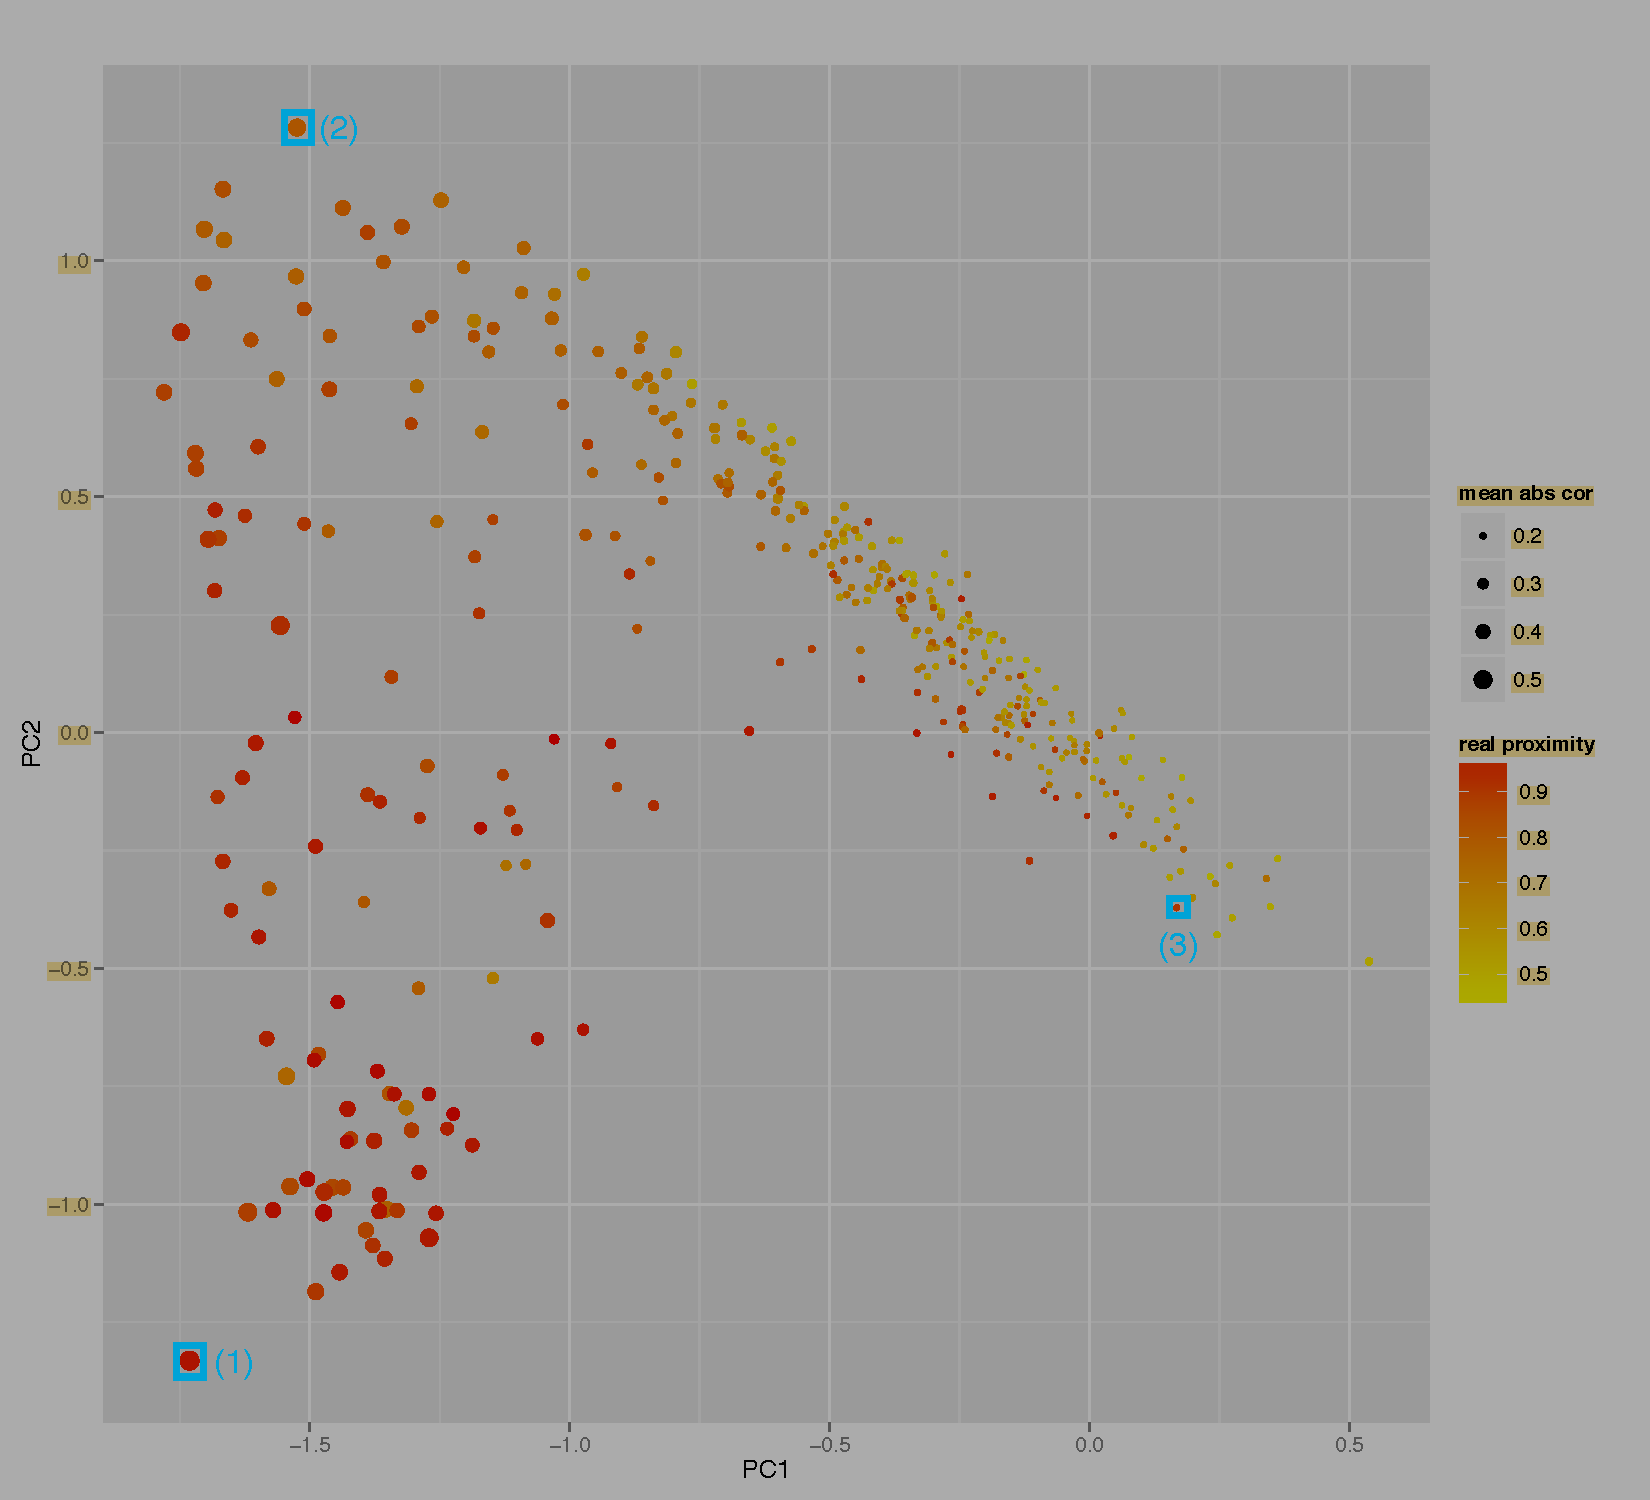
\includegraphics[width=\textwidth]{figures/pca_realDistCol_meanAbsCorSize_withSpecificPoints}
\caption{}
\end{subfigure}
\begin{subfigure}[t]{0.45\linewidth}
\vspace{-8.3cm}
   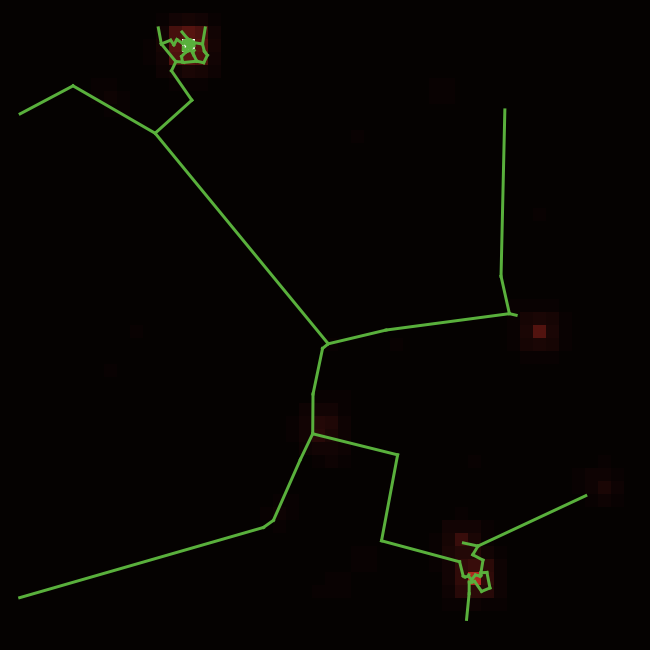
\includegraphics[width=0.49\textwidth]{figures/configs/1_param71861_seed0}
   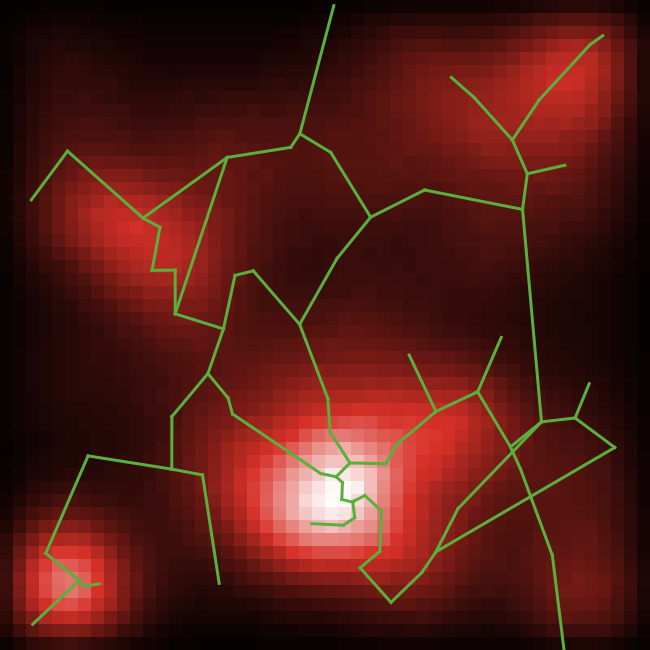
\includegraphics[width=0.49\textwidth]{figures/configs/2_param71913_seed10}\\
   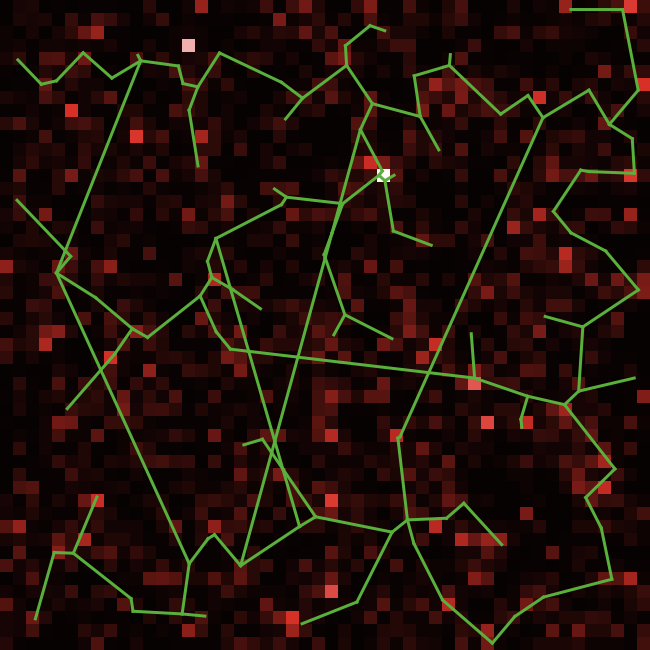
\includegraphics[width=0.49\textwidth]{figures/configs/3_param71918_seed0}
   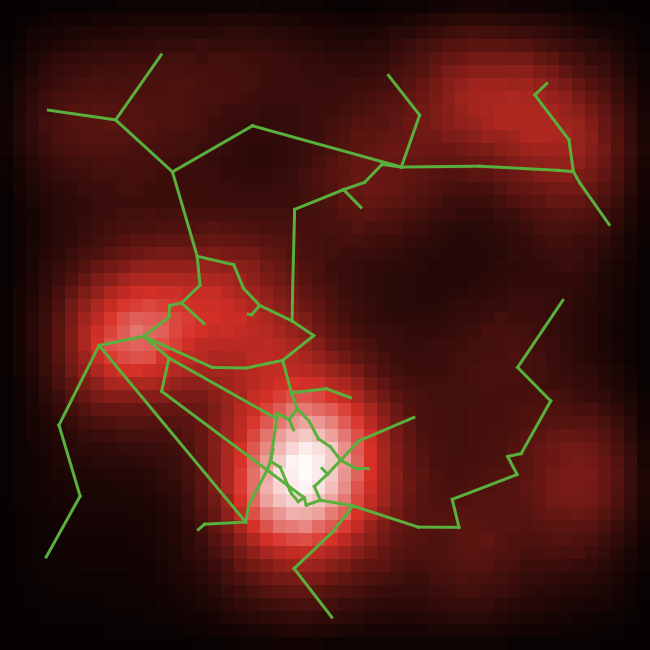
\includegraphics[width=0.49\textwidth]{figures/configs/4_param71945_seed0}
   \caption{}
\end{subfigure}

\caption{\small\textbf{Exploration de l'espace des corrélations entre forme urbaine et réseau | } \textbf{(a)} Distribution des correlations croisées entre les vecteurs $\vec{M}$ des indicateurs morphologiques (dans l'ordre index de moran, distance moyenne, entropie, hiérarchie) et $\vec{N}$ des mesures de réseau (centralité, longueur moyenne, vitesse, diamètre). \textbf{(b)} Amplitude des corrélations, définie comme $a_{ij}=\max_k{\rho_{ij}^{(k)}}-\min_k{\rho_{ij}^{(k)}}$, et correlation absolue maximale, $c_{ij}=\max_k\left| \right|$. \textbf{(c)} Représentation des matrices dans un plan principal obtenu par Analyse en Composantes Principales sur la population des matrices (variances cumulées: PC1=38\%, PC2=68\%). Les barres d'erreur sont calculées initialement par des intervalles de confiance à 95\% sur chaque élément de la matrice (par une méthode de Fisher asymptotique standard), puis les bornes supérieures sont prises dans le plan principal. L'échelle de couleur donne la correlation absolue moyenne sur l'ensemble des variables. \textbf{(d)} }
\label{fig:densnwcor}
\end{figure}
%%%%%%%%%%%%%%



%%%%%%%%%%%%%%
\begin{table}
%regression analysis of param influence on correlations

\end{table}
%%%%%%%%%%%%%%





%%%%%%%%%%%%%%%%%%%%%%
\section{Discussion}
%%%%%%%%%%%%%%%%%%%%%%


%%%%%%%%%%%%%%%%%%%%%%
\subsection{Domaines potentiels d'application}

% ideas of other fields where the generation can happen.



%%%%%%%%%%%%%%%%%%%%%%
\subsection{Positionnement}

% données hybrides au centre de la démarche d'exploration de modèle, analyse de sensitivité etc.






%%%%%%%%%%%%%%%%%%%%%%
\section{Conclusion}
%%%%%%%%%%%%%%%%%%%%%%


On a ainsi proposé une méthode abstraite de génération de données synthétiques corrélées à un niveau contrôlé. Son implémentation partielle dans deux domaines très différents montre sa flexibilité et l'éventail des applications potentielles. De manière générale, il est essentiel de généraliser de telles pratiques de validation systématique de modèles par étude statistique, en particulier pour les modèles agents pour lesquels la question de la validation reste encore relativement ouverte.






\newpage


%%%%%%%%%%%%%%%%%%%%
%% Biblio
%%%%%%%%%%%%%%%%%%%%
\footnotesize

\bibliographystyle{apalike}
\bibliography{/Users/Juste/Documents/ComplexSystems/CityNetwork/Biblio/Bibtex/CityNetwork,biblio/biblio}


\end{document}
